\\documentclass[12pt,a4paper]{article}

%%%%%%%%------------------------------------------------------------------------
%%%% 日常所用宏包

%% 控制页边距
% 如果是beamer文档类, 则不用geometry
\makeatletter
\@ifclassloaded{beamer}{}{\usepackage[top=2.5cm, bottom=2.5cm, left=2.5cm, right=2.5cm]{geometry}}
\makeatother

%% 控制项目列表
\usepackage{enumerate}

%% 多栏显示
\usepackage{multicol}

%% 算法环境
\usepackage{algorithm}  
\usepackage{algorithmic} 
\usepackage{float} 

%% 网址引用
\usepackage{url}

%% 控制矩阵行距
\renewcommand\arraystretch{1.4}

%% hyperref宏包,生成可定位点击的超链接,并且会生成pdf书签
\makeatletter
\@ifclassloaded{beamer}{
\usepackage{hyperref}
\usepackage{ragged2e} % 对齐
}{
\usepackage[%
    pdfstartview=FitH,%
    CJKbookmarks=true,%
    bookmarks=true,%
    bookmarksnumbered=true,%
    bookmarksopen=true,%
    colorlinks=true,%
    citecolor=blue,%
    linkcolor=blue,%
    anchorcolor=green,%
    urlcolor=blue%
]{hyperref}
}
\makeatother



\makeatletter % 如果是 beamer 不需要下面两个包
\@ifclassloaded{beamer}{
\mode<presentation>
{
} 
}{
%% 控制标题
\usepackage{titlesec}
%% 控制目录
\usepackage{titletoc}
}
\makeatother

%% 控制表格样式
\usepackage{booktabs}

%% 控制字体大小
\usepackage{type1cm}

%% 首行缩进,用\noindent取消某段缩进
\usepackage{indentfirst}

%% 支持彩色文本、底色、文本框等
\usepackage{color,xcolor}

%% AMS LaTeX宏包: http://zzg34b.w3.c361.com/package/maths.htm#amssymb
\usepackage{amsmath,amssymb}
%% 多个图形并排
\usepackage{subfig}
%%%% 基本插图方法
%% 图形宏包
\usepackage{graphicx}
\newcommand{\red}[1]{\textcolor{red}{#1}}
\newcommand{\blue}[1]{\structure{#1}}
\newcommand{\brown}[1]{\textcolor{brown}{#1}}
\newcommand{\green}[1]{\textcolor{green}{#1}}


%%%% 基本插图方法结束

%%%% pgf/tikz绘图宏包设置
\usepackage{pgf,tikz}
\usetikzlibrary{shapes,automata,snakes,backgrounds,arrows}
\usetikzlibrary{mindmap}
%% 可以直接在latex文档中使用graphviz/dot语言,
%% 也可以用dot2tex工具将dot文件转换成tex文件再include进来
%% \usepackage[shell,pgf,outputdir={docgraphs/}]{dot2texi}
%%%% pgf/tikz设置结束


\makeatletter % 如果是 beamer 不需要下面两个包
\@ifclassloaded{beamer}{

}{
%%%% fancyhdr设置页眉页脚
%% 页眉页脚宏包
\usepackage{fancyhdr}
%% 页眉页脚风格
\pagestyle{plain}
}

%% 有时会出现\headheight too small的warning
\setlength{\headheight}{15pt}

%% 清空当前页眉页脚的默认设置
%\fancyhf{}
%%%% fancyhdr设置结束


\makeatletter % 对 beamer 要重新设置
\@ifclassloaded{beamer}{

}{
%%%% 设置listings宏包用来粘贴源代码
%% 方便粘贴源代码,部分代码高亮功能
\usepackage{listings}

%% 设置listings宏包的一些全局样式
%% 参考http://hi.baidu.com/shawpinlee/blog/item/9ec431cbae28e41cbe09e6e4.html
\lstset{
showstringspaces=false,              %% 设定是否显示代码之间的空格符号
numbers=left,                        %% 在左边显示行号
numberstyle=\tiny,                   %% 设定行号字体的大小
basicstyle=\footnotesize,                    %% 设定字体大小\tiny, \small, \Large等等
keywordstyle=\color{blue!70}, commentstyle=\color{red!50!green!50!blue!50},
                                     %% 关键字高亮
frame=shadowbox,                     %% 给代码加框
rulesepcolor=\color{red!20!green!20!blue!20},
escapechar=`,                        %% 中文逃逸字符,用于中英混排
xleftmargin=2em,xrightmargin=2em, aboveskip=1em,
breaklines,                          %% 这条命令可以让LaTeX自动将长的代码行换行排版
extendedchars=false                  %% 这一条命令可以解决代码跨页时,章节标题,页眉等汉字不显示的问题
}}
\makeatother
%%%% listings宏包设置结束


%%%% 附录设置
\makeatletter % 对 beamer 要重新设置
\@ifclassloaded{beamer}{

}{
\usepackage[title,titletoc,header]{appendix}
}
\makeatother
%%%% 附录设置结束


%%%% 日常宏包设置结束
%%%%%%%%------------------------------------------------------------------------


%%%%%%%%------------------------------------------------------------------------
%%%% 英文字体设置结束
%% 这里可以加入自己的英文字体设置
%%%%%%%%------------------------------------------------------------------------

%%%%%%%%------------------------------------------------------------------------
%%%% 设置常用字体字号,与MS Word相对应

%% 一号, 1.4倍行距
\newcommand{\yihao}{\fontsize{26pt}{36pt}\selectfont}
%% 二号, 1.25倍行距
\newcommand{\erhao}{\fontsize{22pt}{28pt}\selectfont}
%% 小二, 单倍行距
\newcommand{\xiaoer}{\fontsize{18pt}{18pt}\selectfont}
%% 三号, 1.5倍行距
\newcommand{\sanhao}{\fontsize{16pt}{24pt}\selectfont}
%% 小三, 1.5倍行距
\newcommand{\xiaosan}{\fontsize{15pt}{22pt}\selectfont}
%% 四号, 1.5倍行距
\newcommand{\sihao}{\fontsize{14pt}{21pt}\selectfont}
%% 半四, 1.5倍行距
\newcommand{\bansi}{\fontsize{13pt}{19.5pt}\selectfont}
%% 小四, 1.5倍行距
\newcommand{\xiaosi}{\fontsize{12pt}{18pt}\selectfont}
%% 大五, 单倍行距
\newcommand{\dawu}{\fontsize{11pt}{11pt}\selectfont}
%% 五号, 单倍行距
\newcommand{\wuhao}{\fontsize{10.5pt}{10.5pt}\selectfont}
%%%%%%%%------------------------------------------------------------------------


%% 设定段间距
\setlength{\parskip}{0.5\baselineskip}

%% 设定行距
\linespread{1}


%% 设定正文字体大小
% \renewcommand{\normalsize}{\sihao}

%制作水印
\RequirePackage{draftcopy}
\draftcopyName{XTUMESH}{100}
\draftcopySetGrey{0.90}
\draftcopyPageTransform{40 rotate}
\draftcopyPageX{350}
\draftcopyPageY{80}

%%%% 个性设置结束
%%%%%%%%------------------------------------------------------------------------


%%%%%%%%------------------------------------------------------------------------
%%%% bibtex设置

%% 设定参考文献显示风格
% 下面是几种常见的样式
% * plain: 按字母的顺序排列,比较次序为作者、年度和标题
% * unsrt: 样式同plain,只是按照引用的先后排序
% * alpha: 用作者名首字母+年份后两位作标号,以字母顺序排序
% * abbrv: 类似plain,将月份全拼改为缩写,更显紧凑
% * apalike: 美国心理学学会期刊样式, 引用样式 [Tailper and Zang, 2006]

\makeatletter
\@ifclassloaded{beamer}{
\bibliographystyle{apalike}
}{
\bibliographystyle{unsrt}
}
\makeatother


%%%% bibtex设置结束
%%%%%%%%------------------------------------------------------------------------

%%%%%%%%------------------------------------------------------------------------
%%%% xeCJK相关宏包

\usepackage{xltxtra,fontspec,xunicode}
\usepackage[slantfont, boldfont]{xeCJK} 
\usepackage{bm}

\setlength{\parindent}{2em}%中文缩进两个汉字位

%% 针对中文进行断行
\XeTeXlinebreaklocale "zh"             

%% 给予TeX断行一定自由度
\XeTeXlinebreakskip = 0pt plus 1pt minus 0.1pt

%%%% xeCJK设置结束                                       
%%%%%%%%------------------------------------------------------------------------

%%%%%%%%------------------------------------------------------------------------
%%%% xeCJK字体设置

%% 设置中文标点样式,支持quanjiao、banjiao、kaiming等多种方式
\punctstyle{kaiming}                                        
                                                     
%% 设置缺省中文字体
%\setCJKmainfont[BoldFont={Adobe Heiti Std}, ItalicFont={Adobe Kaiti Std}]{Adobe Song Std}   
\setCJKmainfont{SimSun}
%% 设置中文无衬线字体
%\setCJKsansfont[BoldFont={Adobe Heiti Std}]{Adobe Kaiti Std}  
%% 设置等宽字体
%\setCJKmonofont{Adobe Heiti Std}                            

%% 英文衬线字体
\setmainfont{DejaVu Serif}                                  
%% 英文等宽字体
\setmonofont{DejaVu Sans Mono}                              
%% 英文无衬线字体
\setsansfont{DejaVu Sans}                                   

%% 定义新字体
\setCJKfamilyfont{song}{Adobe Song Std}                     
\setCJKfamilyfont{kai}{Adobe Kaiti Std}
\setCJKfamilyfont{hei}{Adobe Heiti Std}
\setCJKfamilyfont{fangsong}{Adobe Fangsong Std}
\setCJKfamilyfont{lisu}{LiSu}
\setCJKfamilyfont{youyuan}{YouYuan}

%% 自定义宋体
\newcommand{\song}{\CJKfamily{song}}                       
%% 自定义楷体
\newcommand{\kai}{\CJKfamily{kai}}                         
%% 自定义黑体
\newcommand{\hei}{\CJKfamily{hei}}                         
%% 自定义仿宋体
\newcommand{\fangsong}{\CJKfamily{fangsong}}               
%% 自定义隶书
\newcommand{\lisu}{\CJKfamily{lisu}}                       
%% 自定义幼圆
\newcommand{\youyuan}{\CJKfamily{youyuan}}                 

%%%% xeCJK字体设置结束
%%%%%%%%------------------------------------------------------------------------

%%%%%%%%------------------------------------------------------------------------
%%%% 一些关于中文文档的重定义
\newcommand{\chntoday}{\number\year\,年\,\number\month\,月\,\number\day\,日}
%% 数学公式定理的重定义

%% 中文破折号,据说来自清华模板
\newcommand{\pozhehao}{\kern0.3ex\rule[0.8ex]{2em}{0.1ex}\kern0.3ex}

\newtheorem{example}{例}                                   
\newtheorem{theorem}{定理}[section]                         
\newtheorem{definition}{定义}
\newtheorem{axiom}{公理}
\newtheorem{property}{性质}
\newtheorem{proposition}{命题}
\newtheorem{lemma}{引理}
\newtheorem{corollary}{推论}
\newtheorem{remark}{注解}
\newtheorem{condition}{条件}
\newtheorem{conclusion}{结论}
\newtheorem{assumption}{假设}

\makeatletter %
\@ifclassloaded{beamer}{

}{
%% 章节等名称重定义
\renewcommand{\contentsname}{目录}     
\renewcommand{\indexname}{索引}
\renewcommand{\listfigurename}{插图目录}
\renewcommand{\listtablename}{表格目录}
\renewcommand{\appendixname}{附录}
\renewcommand{\appendixpagename}{附录}
\renewcommand{\appendixtocname}{附录}
%% 设置chapter、section与subsection的格式
\titleformat{\chapter}{\centering\huge}{第\thechapter{}章}{1em}{\textbf}
\titleformat{\section}{\centering\sihao}{\thesection}{1em}{\textbf}
\titleformat{\subsection}{\xiaosi}{\thesubsection}{1em}{\textbf}
\titleformat{\subsubsection}{\xiaosi}{\thesubsubsection}{1em}{\textbf}

\@ifclassloaded{book}{

}{
\renewcommand{\abstractname}{摘要}
}
}
\makeatother

\renewcommand{\figurename}{图}
\renewcommand{\tablename}{表}

\makeatletter
\@ifclassloaded{book}{
\renewcommand{\bibname}{参考文献}
}{
\renewcommand{\refname}{参考文献} 
}
\makeatother

\floatname{algorithm}{算法}
\renewcommand{\algorithmicrequire}{\textbf{输入:}}
\renewcommand{\algorithmicensure}{\textbf{输出:}}

%%%% 中文重定义结束
%%%%%%%%------------------------------------------------------------------------

\begin{document}

\title{时变偏微分方程的隐式显式Runge-Kutta方法}
\author{Uri M. Ascher , Steven J. Ruuth, Raymond J. Spiteri}
\date{1997}
\maketitle

\textbf{摘要}
用于偏微分方程的隐式显式(IMEX)线性多步时间离散格式已经证明在许多应用中是有用的。然而,当应用于对流扩散问题时,它们倾向于具有不良的时间步长限制,除非扩散强烈占优,并且选择适当的基于BDF的格式。在本文中,我们发展了基于Runge-Kutta-的IMEX格式,它比较著名的是IMEX多步格式在大参数范围内具有更好的稳定区域。

\section{介绍}
当时变偏微分方程(PDE)涉及不同类型的项时,对它们采用不同的离散。隐式显式(IMEX)时间离散格式就是这种策略的一个例子。线性多步IMEX格式已被许多研究者所采用,特别是与谱方法相结合的方法[3,10]。在20世纪70年代末,提出并分析了这种类型的一些格式[5,15]。这些方法的实例已成功应用于不可压缩的Navier-Stokes方程[9]和环境模拟研究[16]。文献[2]对对流-扩散型偏微分方程进行了比较系统的研究,文献[11]报道了形态学上反应扩散问题的相应的研究。

在这项工作中,我们考虑对流扩散型(或双曲抛物型方程)的问题,例如:
\begin{equation}
u_{t}=uu_{x}+\nu\Delta u,~~~\nu >0.
\label{11}
\end{equation}
空间导数的离散(例如,通过有限差分、有限元、有限体积或谱方法)在时间上产生非常大的ODE系统
\begin{equation}
\dot{u}=f(u)+g(u),
\label{12}
\end{equation}
其中$f$对应于对流(双曲线)项$uu_{x}$,$g$对应于扩散(抛物线)项$\nu\Delta u$。IMEX格式包括$g$的隐式离散和$f$的显式离散。这是自然的,因为$f\equiv 0$时(\ref{12})通常是刚的的和线性的,而在$g\equiv 0$的情况下,系统不是刚的,和通常是非线性的。此外,如果对后一种情况坚持使用隐式离散,通过矩阵逆的性质构造迭代求解器是个巨大挑战。

在[2]中,我们对(\ref{12})的线性多步格式进行了分析和实验。对于扩散占优问题,$g$有最优阻尼特性采用向后差分(BDF)种格式。相应的IMEX格式是半显式BDF(SBDF)[5,9,15]。然而,当扩散不占优时,方法的选择就不那么明显了。理想情况下,人们希望双曲项是耗散格式,以便得到IMEX格式具有良好的稳定性和平滑性,与$g(u)$无关。然而,众所周知,寻找3阶(或更准确地说,向后步骤)以上的格式非常必要参见[2]。多步IMEX格式的主要困难是由于稳定性限制需要相对较小的时间步长(例如,[14])。使用高阶多步格式时,这种限制会变得更差,如[2]中所示。另一方面,当考虑三阶和四阶格式时,显式Runge-Kutta格式的稳定性区域实际上有所增加。因此,我们研究IMEX Runge-Kutta格式的发展和性能。

当(\ref{12})来自多个空间变量的PDE时,在每个时间步长离散隐式部分相对应的代数方程的简单性和效率是至关重要的。在[2]中,我们表明,在适当的情况下和某些IMEX格式中,每个时间步长不需要多于一个多重网格W循环。在这里,我们研究是每个Runge-Kutta级的性质。 因此,我们专注$g(u)$的对角隐式Runge-Kutta(DIRK)格式,特别注意它们的衰减特性。我们构建了许多此类IMEX格式,并研究它们的属性。对于非常刚的ODEs DIRK格式的阶降到1[8],在$g(u)$占主导地位且非常刚性时我们不期望Runge-Kutta格式与SBDF进行极限比较。然而,我们的Runge-Kutta格式对于其它参数范围有优越的性能。

众所周知,使用Runge-Kutta格式整合时变的偏微分方法并不是没有缺点。问题一是,当给定时变流入边界条件时,精度会下降[4]。[1]中提出了一种补救措施。还要注意的是,在最后一步的精确性高于内部阶段,必须计算这些内部阶段不能降低的精确性(例如通过迭代方法,如第5节中所述)。

(\ref{12})可以转换为分区体系
\begin{gather*}
\dot{v}=\widehat{f}(v,w),
\label{131} \\
\dot{w}=\widehat{g}(v,w),
\label{132}
\end{gather*}
其中$u=v+w,\widehat{f}=f(v+w)$和$\widehat{g}=g(v+w)$下面设计的IMEX Runge-Kutta格式是分段的Runge-Kutta格式。 他们的阶在[7,第II.15节]中讨论。它们也可以被视为一种特殊的分裂方法。我们注意到对于(\ref{12}),$v$和$w$不需要单独知道(实际上,我们可能没有它们的初始条件)。我们所需要的是它们的光滑性和局部存在性。

在第二节中,我们开发了多达四级的IMEX Runge-Kutta格式,其精度可达三阶。这些格式划分为两类--在下一个时间处(即在时间步长的末尾)解决最后一个内部阶段,以及在步骤结束处使用附加正交。第一类特别适用于高度刚性的问题,但第二类似乎为广泛参数提供了一些比较有前途的变体,特别是被定义为(3,4,3)(隐式公式为内部3级,显式为4级和综合精度为3阶)的格式。

在第3节中,我们研究了一个简单测试方程各种格式的性能,这些方程来自对流扩散方程的冯诺依曼分析。稳定区域绘制在图1和2中。线性对流-扩散方程的试验结果在4.1节中呈现,Burgers方程在4.2节中进行了实验。在第5节中,我们研究了各种格式的性能,并结合使用多重网格方法来解决每个阶段的隐性。


\section{IMEX Runge-Kutta 格式}
设初值问题
\begin{equation*}
\begin{cases}
u^{'}=f(t,u),\\
u(t_{0})=u_{0}
\end{cases}
\end{equation*}
的解充分光滑,将$u(t)$在$t_{0}$处用泰勒展开:
\begin{equation*}
u(t_{1})=u(t_{0})+hu^{'}(t_{0})+\frac{h^2}{2!}u^{(2)}(t_{0})+\cdots+\frac{h^{(p)}}{p!}(t_{0})+O(h^{p+1})
\end{equation*}
其中$u(t_{0})=u_{0},u^{'}(t_{0})=f(t_{0},u(t_{0}))=f(t_{0},u_{0})$\\
令
\begin{equation*}
\varphi(t,u(t),h)=\sum_{j=1}^{p}\frac{h^{j-1}}{j!}\frac{d^{j-1}}{dt^{j-1}}f(f,u(t))
\end{equation*}
则上面泰勒展开式子可以写成:
\begin{equation*}
u(t_{0}+h)-u(t_{0})=h\varphi(t_{0},h(t_{0}),h)+O(h^{p+1})
\end{equation*}
龙格库塔的一般格式:
\begin{gather*}
u_{n+1}=u_{n}+h\varphi(t_{n},u_{n},h),~n=0,1,\cdots
\end{gather*}
其中
\begin{gather}
\varphi(t,u(t),h)=\sum_{i=1}^{m}b_{i}k_{i}
\end{gather}
\begin{equation}
\begin{cases}
k_{1}=f(t,u)\\
k_{2}=f(t+hc_{2},u(t)+ha_{21}k_{1})\\
\cdots\cdots\\
k_{m}=f(t+hc_{m},u(t)+h\sum_{j=1}^{m-1}a_{mj}k_{j})
\end{cases}
\sum_{j=1}^{i-1}a_{ij}=c_{i},~~~~\sum_{i=1}^{m}b_{i}=1
\end{equation}
为了确定$\{a_{ij}\},\{b_{j}\},\{c_{i}\}$的系数,我们将$u(t+h)$展开到$h$的三次幂
\begin{equation*}
u(t+h)=u(t)+\sum_{l=1}^{3}\frac{h^l}{l!}u^{l}(t)+O(h^4)=u(t)+h\varphi_{T}(t,u,h)
\end{equation*}
其中
\begin{align*}
&\varphi_{T}(t,u,h)=u^{(1)}(t)+\frac{1}{2!}hu^{(2)}(t)+\frac{1}{3!}h^2u^{(3)}(t)+O(h^4)\\
&=f+\frac{1}{2}hF+\frac{1}{6}h^2(Ff_{u}+G)+O(h^3)\\
&F=f_{t}+ff_{u}\\
&G=f_{tt}+2ff_{tu}+f^2f_{uu}
\end{align*}
由二元泰勒展开:
\begin{equation*}
k_{1}=f(t,u)=f;
\end{equation*}
\begin{align*}
k_{2}&=f(t+hc_{2},u+ha_{21}k_{1})\\
&=f+hc_{2}f_{t}+ha_{21}k_{1}f_{u}+\frac{1}{2}h^2(c_{2}^2f_{tt}+2c_{2}a_{21}f_{tu}+(a_{21}k_{1})^2f_{uu})+O(h^3)\\
&=f+hc_{2}F+\frac{1}{2}h^2c_{2}^2G+O(h^3)
\end{align*}
同理得:
\begin{equation*}
k_{3}=f+hc_{3}F+h^2(c_{2}a_{32}f_{u}F+\frac{1}{2}c_{3}^2G)+O(h^3).
\end{equation*}
\begin{align*}
\varphi(t,u,h)=&(b_{1}+b_{2}+b_{3})f+h(c_{2}b_{2}+c_{3}b_{3})F+\\
&\frac{1}{2}h^2\biggl[2c_{2}a_{32}b_{3}f_{u}F+(c_{2}^2b_{2}+c_{3}^2b_{3})G\biggr]+O(h^3)
\end{align*}
比较$\varphi(t,u,h)$和$\varphi_{T}(t,u,h)$同次幂系数,当$m=3$时,有
\begin{gather*}
b_{1}+b_{2}+b_{3}=1,~~~c_{2}b_{2}+c_{3}b_{3}=\frac{1}{2},\\
c_{2}^2b_{2}+c_{3}^2b_{3}=\frac{1}{3},~~~c_{2}a_{32}b_{3}=\frac{1}{6}
\end{gather*}



我们现在发展一些IMEX龙格-库塔格式。对于$g$,我们在通常的Butcher表示法中考虑系数$A\in R^{s\times s} ,c,b\in R^s$的隐式$s$级DIRK格式[8]。令$\sigma=s+1$。对于$f$,我们考虑一个$(s+1)$级显式格式,其中横坐标$\widehat{c}=\binom{0}{c}$和系数$\widehat{A}\in R^{\sigma\times \sigma},\widehat{b}\in
R^{\sigma}.$为了将DIRK格式转换为$(s+1)$级格式,我们可以用零填充s级格式,获得
\[
\begin{array}{r|r r r r  r}
0 &  0 & 0 & 0  & \cdots & 0 \\
c_{1} & 0 & a_{11} & 0 & \cdots & 0 \\
c_{2} & 0 & a_{21} & a_{22} & \cdots & 0 \\
\vdots & \vdots &  \vdots &  &  \ddots &  \vdots \\
c_{s} & 0 & a_{s1} & a_{s2} & \cdots & a_{ss} \\
\hline
 & 0 & b_{1} & b_{2} & \cdots & b_{s} 
\end{array}
\]
参考这个填充的系数为$\tilde{A}\in R^{\sigma\times\sigma},\tilde{b}\in R^{\sigma},\tilde{c}\in R^{\sigma}$我们发现$\tilde{c}=\widehat{c}$。由于各格式之间耦合的性质简化了系数上阶条件的形式。

IMEX格式$t_{n-1}$到$t_{n}=t_{n-1}+k$的一步给出如下:

令:

\begin{equation}
\widehat{K_{1}}=f(u_{n}-1),
\label{211}
\end{equation}
对$i=1,\cdots,s$:

\textbullet 解决$K_{i}$:
\begin{equation}
K_{i}=g(u_{i}),
\label{212}
\end{equation}

其中

\begin{equation}
u_{i}=u_{n-1}+k\sum_{j=1}^{i}a_{i,j}K_{j}+k\sum_{j=1}^{i}\widehat{a}_{i+1,j}\widehat{K}_{j}.
\label{213}
\end{equation}

\textbullet 估计

\begin{equation}
\widehat{K}_{i+1}=f(u_{i}).
\label{214}
\end{equation}
最后,估计
\begin{equation}
u_{n}=u_{n-1}+k\sum_{j=1}^{s}b_{j}K_{j}+k\sum_{j=1}^{\sigma}\widehat{b}_{j}\widehat{K}_{j}.
\label{215}
\end{equation}

我们考虑了两类特殊情况,引出俩个子系列的方法:满足(\ref{22})和满足(\ref{23})-(\ref{24}):

(1)在$\widehat{b}=\tilde{b}$(特别是$\widehat{b}_{1}=0$)我们代替(\ref{215})
\begin{equation}
u_{n}=u_{n-1}+k\sum_{j=1}^{s}b_{j}(K_{j}+\widehat{K}_{j+1})
\label{22}
\end{equation}

(2)在$\widehat{b}_{s+1}=0,\widehat{K}_{s+1}$不需要估计,如果:
\begin{equation}
b_{j}=a_{s,j},~~\widehat{b}_{j}=\widehat{a}_{s+1,j},~~~~j=1,\cdots,s
\label{23}
\end{equation}
(暗示隐式格式是精确的并且$c_{s}=1$),然后将(\ref{215})代入$u_{s}$的表达式,我们看到了
\begin{equation}
u_{n}=u_{s}
\label{24}
\end{equation}
这对刚性的问题很有用。我们还注意到显式格式可以基于横坐标$c_{1},\cdots,c_{s-1}$的一般显式s级格式生成
\[
\begin{array}{r|r r r r r}
0 & 0 & 0 & 0 & \cdots & 0\\
c_{1}  & \widehat{a}_{21} & 0 & 0 & \cdots & 0\\
c_{2}  & \widehat{a}_{31} & \widehat{a}_{32} & 0 & \cdots & 0\\\
\vdots & \vdots & \vdots & \vdots & \ddots & 0\\
c_{s-1}  & \widehat{a}_{s1} & \widehat{a}_{s2} & \widehat{a}_{s3} & \cdots & 0\\
\hline
& \widehat{b}_{1} & \widehat{b}_{2} & \widehat{b}_{3} & \cdots & \widehat{b}_{s}
\end{array}
\]

在(\ref{212})中,有$s$个非线性系统需要$g$单独求解,而要转置的算子是
\begin{equation}
I-ka_{ii}g_{u}
\end{equation}
假设雅可比$g(u)$仅被评估一次(在$t_{n-1}$),如果$a_{ii}$独立于$i$,即对于SDIRK格式,则该算子对于每个i是相同的。然而,如果将诸如1个周期多重网格的迭代方法用于隐式格式,则可能对于SDIRK的整体效率不太重要,并且可以考虑更一般的DIRK格式。有关刚性精确的SDIRK格式,请参见[8,第IV.6节]。在我们寻找准确和稳定的格式时,我们允许A的对角元素彼此不同。尽管如此,我们推荐的格式都是SDIRK,因为在解决过程中有足够的自由度来选择计算效率。

\textbf{例 1}~考虑(\ref{12})的情况,其中

\begin{equation}
u=\binom{q}{p},~~~f=\binom{0}{f_{2}},~~~g=\binom{f_{1}}{0}
\end{equation}
因此,我们应用隐式格式来推进$q$,使用显式方法来推进$p$。如果$f_{2}$受控制函数的影响,那么在每个级$i$,这种影响将$K_{i}$传播到$\widehat{K}_{i}$。使用“正常”显式格式时不会发生这种情况(参见[13])。而且,如果$f_{1}$与$q$无关,则

\begin{equation}
I-ka_{ii}g_{u}=\left(
\begin{array}{c c}
I & -ka_{ii}(f_{1})_{p}\\
0 & I\\
\end{array}
\right)
\end{equation}
这个格式就变成显示的了!

特别是对于哈密顿体系,我们可以设$u=(q,p)^T,f=(0,-H_{q})^T,~g=(H_{p},0)^T$。如果$H_{p}$独立于q,则得到一个显式格式,它仍然保留了隐式格式的一些优点。


我们现在构建IMEX RK簇格式一些实例。我们将使用三元组$(s,\sigma,p)$来识别格式(\ref{211})-(\ref{215}),其中s是隐式格式的级数,$\sigma$是显式格式级数(因此,对于情况(1)$\sigma=s+1$,例如(\ref{22}),对于情况(2)$\sigma=s$对于情况(2),例如(\ref{23})和(\ref{24}),p是该格式的组合阶。


龙格库塔P阶相容的充要条件是对于一切不高于p阶的带根树$t\in T$,有
\begin{equation*}
\phi(t)=\frac{1}{r(t)}
\end{equation*}
其中$r(t)$为t的一切子数的顶点数的乘积。

龙格库塔4阶相容的充要条件:
\begin{equation*}
\phi(t)=\frac{1}{r(t)} ~~~t\in T,r(t)\le 4
\end{equation*}
或者
\begin{align*}
&\tau~~~~\sum_{j=1}^{s}b_{j}=1,\\
&t_{2}~~~~\sum_{j=1}^{s}b_{j}c_{j}=\frac{1}{2},\\
&t_{31}~~~~\sum_{j=1}^{s}b_{j}c_{j}^2=\frac{1}{3},\\
&t_{32}~~~~\sum_{j,k=1}^{s}b_{j}a_{jk}c_{k}=\frac{1}{6}\\
&t_{41}~~~~\sum_{j=1}^{s}b_{j}c_{j}^3=\frac{1}{4}\\
&t_{42}~~~~\sum_{j,k=1}^{s}b_{j}a_{jk}c_{k}c_{j}=\frac{1}{8}\\
&t_{43}~~~~~\sum_{j,k=1}^{s}b_{j}a_{jk}c_{k}^2=\frac{1}{12}\\
&t_{44}~~~~~\sum_{j,k,l=1}^{s}b_{j}a_{jk}a_{kl}c_{l}=\frac{1}{24}
\end{align*}
\subsection{向前向后欧拉(1,1,1)}

这对向后和向前欧拉格式:
\[
\begin{array}{r|r}
1 & 1 \\
\hline
& 1
\end{array},~~~~~~~~~~~~~~~~~~~~~~~
\begin{array}{r|r}
0 & 0 \\
\hline
& 1 
\end{array}
\]
可以填充为:
\[
\begin{array}{r|rr}
0 & 0 & 0 \\
1 & 0 & 1 \\
\hline
& 0 & 1
\end{array},~~~~~~~~~~~~~~~~
\begin{array}{r|rr}
0 & 0 & 0\\
1 & 1 & 0\\
\hline
& 1 & 0
\end{array}.
\]
\begin{gather*}
u_{1}=u_{n-1}+ka_{11}k_{1}+k\hat{a}_{21}\hat{k}_{1}=u_{n-1}+k k_{1}+k \hat{k}_{1}\\
k_{1}=g(u_{1})\\
\hat{k}_{1}=f(u_{n-1})
\end{gather*}
所以
\begin{equation*}
u_{1}=u_{n-1}+k(g(u_{1})+f(u_{n-1}))
\end{equation*}

\begin{equation*}
u_{n}=u_{n-1}+k(b_{1}k_{1}+\hat{b}_{1}\hat{k}_{1})=u_{n-1}+kk_{1}+k\hat{k}_{1}
\end{equation*}
即
\begin{equation*}
u_{n}=u_{n-1}+k(g(u_{1})+f(u_{n-1}))
\end{equation*}
这产生线性一步IMEX(参见[2]):
\begin{equation}
u_{n}=u_{n-1}+k(f(u_{n-1}))+g(u_{n})).
\end{equation}
该格式满足(\ref{23})。

\subsection{向前向后欧拉(1,2,1)}

上述形式的欧拉方法不满足$\widehat{b}=\tilde{b}$。做变体之后是:
\[
\begin{array}{r|rr}
0 & 0 & 0\\
1 & 0 & 1 \\
\hline
& 0 & 1
\end{array},~~~~~~
\begin{array}{r|rr}
0 & 0 & 0\\
1 & 1 & 0 \\
\hline
& 0 & 1
\end{array}
\]

\begin{gather}
u_{1}=u_{n-1}+ka_{11}k_{1}+k\hat{a}_{21}\hat{k}_{1}=u_{n-1}+k(g(u_{1})+f(u_{n-1}))
\end{gather}
\begin{equation*}
u_{n}=u_{n-1}+k(b_{1}g(u_{1})+\hat{b}_{2}f(u_{1}))=u_{n-1}+k(g(u_{1})+f(u_{1}))
\end{equation*}
例如:$(u_{n}=u_{n-1}+k(g(u_{1})+f(u_{1}))$其中$u_{1}=u_{n-1}+kg(u_{1})+kf(u_{n-1})$与以前的格式相比,该格式每步需要对f进行额外的评估。

\subsection{隐式显式中点(1,2,2)}
欧拉对是一阶精确的,当$g=0$(参见[2]的第三部分)时,(1,1,1)格式有着众所周知的缺点。下列一对隐式显式格式:
\[
\begin{array}{r|rr}
0 & 0 & 0\\
\frac{1}{2} & 0 & \frac{1}{2}\\
\hline
& 0 & 1
\end{array},~~~~~~~~~~~~~~
\begin{array}{r|rr}
0 & 0 & 0\\
\frac{1}{2} & \frac{1}{2} & 0\\
\hline
& 0 & 1
\end{array}
\]

\begin{equation*}
u_{1}=u_{n-1}+ka_{11}k_{1}+k\hat{a}_{21}\hat{k}_{1}=u_{n-1}+\frac{k}{2}(k_{1}+\hat{k}_{1})
\end{equation*}
即
\begin{equation*}
u_{1}=u_{n-1}+\frac{k}{2}(g(u_{1})+f(u_{n-1}))
\end{equation*}
\begin{equation*}
u_{n}=u_{n-1}+kb_{1}k_{1}+k\hat{b}_{2}\hat{k}_{2}
\end{equation*}
即
\begin{equation*}
u_{n}=u_{n-1}+k(g(u_{1})+f(u_{1}))
\end{equation*}
应用于f的显式中点和g的隐式中点。它是二阶精确的,因为它组成的两个格式都是二阶精确的和$\widehat{c}=\tilde{c}[7]$该格式与文献[2]中所考虑的不合理的CNAB格式相比,具有较好的对称性。

\textbf{例2}将格式(1,2,2)应用于可分哈密顿体系
\begin{equation}
\dot{q}=H_{p}(p),~~~~~~~~~~~~~\dot{p}=-H_{q}(q)
\end{equation}
定义
\begin{equation}
u=\binom{q}{p},~~~f=\binom{H_{p}}{0},~~~~g=\binom{0}{-H_{q}},
\end{equation}
我们得到
\begin{align}
&\widehat{K}_{1}=f(u_{n-1})=\binom{H_{p}(p_{n-1})}{0},~~K_{1}=g(u_{1})=\binom{0}{-H_{q}(q_{1})},\\
&\binom{q_{1}}{p_{1}}=\binom{q_{n-1}}{p_{n-1}}+\frac{k}{2}(K_{1}+\widehat{K}_{1})=\binom{q_{n-1}}{p_{n-1}}+\frac{k}{2}\binom{H_{p}(p_{n-1})}{-H_{q}(q_{1})},\\
&\widehat{K}_{2}=f(u_{1})=\binom{H_{p}(p_{1})}{0},~~~~~~\binom{q_{n}}{p_{n}}=\binom{q_{n-1}}{p_{n-1}}+k(K_{1}+\widehat{K}_{2})=\binom{q_{n-1}}{p_{n-1}}+k\binom{H_{p}(p_{1})}{-H_{q}(q_{1})}
\end{align}
我们注意到这个格式是显示的,它也可以表示为辛。 它与跳蛙/ Verlet格式相同[12] 
\begin{gather}
p_{n}=p_{n-1}-kH_{q}(q_{n-1}+\frac{k}{2}H_{p}(p_{n-1})),\\
q_{n}=q_{n-1}+kH_{p}\bigg(\frac{p_{n}+p_{n-1}}{2}\biggl).
\end{gather}
\subsection{三阶组合(2,3,3)}
s级单隐龙格库塔的稳定函数:
\begin{equation*}
R(z)=\frac{p(z)}{(1-\lambda z)^s}
\end{equation*}
$p(z)$是不超过s次多项式,这里$\lambda$是Runge-Kutta矩阵的s重非零实特征值。

阶$p\ge s$的s级单隐Runge-Kutta法的稳定函数$R(z)$的分子可以表示为:
\begin{equation*}
p(z)=\sum_{i=0}^{s}\bigg(\sum_{j=0}^{i}\frac{(-1)^j}{(i-j)!}\binom{s}{j}\lambda^j\biggl)z^i
\end{equation*}
当$p=s$时,$R(z)$作为$exp(z)$的$p$阶有理逼近,误差常数为:
\begin{equation*}
C=\sum_{j=0}^{s}\frac{1}{(s+1-j)!}(-\lambda)^j\binom{s}{j}\ne 0;
\end{equation*}
若$C=0$,则有理逼近达到最大阶$p=s+1$。

具有最佳阻尼特性的二级三阶DIRK格式是DIRK格式[7,p.207]
\begin{equation*}
C=\lambda^2-\lambda+\frac{1}{6}
\end{equation*}
\begin{gather*}
p(z)=1+z-2\lambda z+\frac{1}{2}z^2-2\lambda z^2+\lambda^2z^2\\
\end{gather*}
\begin{equation*}
R(\infty)=\lim\limits_{z\to \infty}R(z)=\frac{\frac{1}{2}-2\lambda+\lambda^2}{\lambda^2}
\end{equation*}
\[
\begin{array}{r|rr}
\gamma & \gamma & 0 \\
1-\gamma & 1-2\gamma & \gamma  \\
\hline
& \frac{1}{2} & \frac{1}{2}
\end{array}
\]
其中$\gamma=(3+\sqrt{3})/6$,对于测试公式$\dot{u}=\alpha u$,如果令$z=\alpha k$,当$z\to -\infty,R(\infty)=1-\sqrt{3}\approx -0.7321.$这是对中点格式(1,2,2)的显着改进,其在刚度极限$\infty$处没有衰减。

相应的三阶显式Runge-Kutta格式(ERK)是
\[
\begin{array}{r|rrr}
0 & 0 & 0 & 0\\
\gamma & \gamma & 0 & 0\\
1-\gamma & \gamma -1 & 2(1-\gamma ) & 0\\
\hline
& 0 & \frac{1}{2} & \frac{1}{2}
\end{array}
\]
得到的IMEX组合是三阶精确的,在虚轴附近有些耗散(就像所有三阶ERK方法一样),并且在$\infty$处有一些稳定函数的衰减。

设初值问题
\begin{equation*}
\begin{cases}
u^{'}=f(t,u),\\
u(t_{0})=u_{0}
\end{cases}
\end{equation*}
求初值问题形如:
\begin{equation}
\sum_{i=0}^{k}\alpha_{i}y_{n+i}=h\varphi_{f}(t_{n};y_{n},y_{n+1},\cdots,y_{n+1};h)~~n=0,\cdots,N-k
\label{27}
\end{equation}
的方法,称为一般多步法,其中$h>0$是积分步长,$k\ge 1$是方程的步数。

(Dahquist提出)方法(\ref{27})称为是A-稳定的,如果满足:
\begin{equation*}
S\supset C_{\_}=\{\bar{h}\in C|Re\bar{h}<0\}.
\end{equation*}
方法(\ref{27})称为是L-稳定的,如果它是A-稳定的,且在$\infty$点极端稳定。

单步方法L-稳定性定义由Ehle首先提出。

龙格库塔法A-稳定的充要条件是其稳定函数$R(z)$于复平面$\{z\in C|Rez<0\}$是解析的,且满足
\begin{equation}
|R(iy)|\le 1,~~y\in R
\end{equation}

一个方法是L-稳定的,如果满足A-稳定和
\begin{equation*}
\lim\limits_{z\to\infty}R(z)=0
\end{equation*}
\subsection{L稳定,二级,二阶DIRK(2,3,2)}

可能有人认为,上述格式所具有的衰减可能不足以解决某些问题。一个两级,二阶DIRK格式,其刚性非常准确[8,p.106]
\begin{gather*}
p(z)=1+z-2\lambda z+\frac{1}{2}z^2-2\lambda z^2+\lambda^2z^2\\
\end{gather*}
\begin{equation*}
R(\infty)=\lim\limits_{z\to \infty}R(z)=\frac{\frac{1}{2}-2\lambda+\lambda^2}{\lambda^2}
\end{equation*}
\[
\begin{array}{r|rr}
\gamma & \gamma & 0\\1 & 1-\gamma & \gamma\\
\hline
& 1-\gamma & \gamma
\end{array}
\]
其中$\gamma=(2-\sqrt{2})/2$。相应的三级二阶ERK是
\[
\begin{array}{r|rrr}
0 & 0 & 0 & 0\\
\gamma & \gamma & 0 & 0 \\
1 & \delta& 1-\delta & 0\\
\hline
& 0 & 1-\gamma & \gamma
\end{array}
\]
改变$\delta$以得到耗散稳定区域,我们将稳定性函数中指数的项提高到三阶。这产生三级,三阶显式RK格式的稳定性区域,其中$\delta=-2\sqrt{2}/3$。得到的IMEX组合是二阶精确的。

\subsection{L稳定,两级,二阶DIRK(2,2,2)}

我们使用与之前的IMEX格式相同的形式(具有相同的$\gamma$但$\delta$尚未指定),除了要求(\ref{23})代替(\ref{22})。例如:$\widehat{b}_{1}=\delta,\widehat{b}_{2}=1-\delta,\widehat{b}_{3}=0$。这给出了二阶格式

\[
\begin{array}{r|rr}
\gamma & \gamma & 0\\
1 & 1-\gamma & \gamma \\
\hline
&1-\gamma & \gamma 
\end{array}~~~~~~~~~~~~
\begin{array}{r|rrr}
0 & 0 & 0 & 0 \\
\gamma & \gamma & 0 & 0\\
1 & \delta & 1-\delta & 0\\
\hline
& \delta & 1-\delta & 0
\end{array}
\]
其中$\delta=1-1/(2\gamma)$.

\subsection{L稳定,3级,3阶DIRK(3,4,3)}

我们现在想开发更大的耗散区域,其中在虚轴附近四级,四阶ERK格式。三级,三阶DIRK格式,非常准确[8,p.106]
\[
\begin{array}{r|rrr}
\gamma & \gamma & 0 & 0\\
\frac{1+\gamma }{2} & \frac{1-\gamma }{2} & \gamma  & 0 \\
1 & b_{1}(\gamma ) &  b_{2}(\gamma ) & \gamma \\
\hline
&  b_{1}(\gamma ) &  b_{2}(\gamma ) &\gamma
\end{array}
\]
其中$\gamma$是$6x^3-18x^2+9x-1=0$中点的根。\\
$b_{1}(\gamma)=-\frac{3}{2}\gamma^2+4\gamma-\frac{1}{4}$和$b_{2}(\gamma)=\frac{3}{2}\gamma^2-5\gamma+\frac{5}{4}$\\
数值估计
\[
\begin{array}{r|rrr}
0.43586652115 & 0.4358665215 & 0 & 0\\
0.7179332608 &0.2820667392 & 0.4358665215 & 0\\
1 & 1.208496649 & -0.644363171 & 0.4358665215 \\
\hline
& 1.208496649 & -0.644363171 & 0.4358665215
\end{array}
\]
构造相应的四级三阶ERK,使得它与所有四级,四阶ERK格式有相同的稳定区域:
\[
\begin{array}{r|rrrr}
0 & 0 & 0 & 0 & 0 \\
\gamma & \gamma & 0 & 0 & 0\\
\frac{1+\gamma}{2} & \widehat{a}_{31}(\gamma) & \widehat{a}_{32}(\gamma) & 0 & 0\\
1 & \widehat{a}_{41}(\gamma) & \widehat{a}_{42}(\gamma) & \widehat{a}_{43}(\gamma) & 0\\
\hline
& 0 & b_{1}(\gamma) & b_{2}(\gamma) & \gamma 
\end{array}
\]
三阶条件表明这是一个双参数族格式。把我们的自由度变成$\widehat{a}_{42},\widehat{a}_{43}$,其余的表达方式都是
\begin{gather}
\widehat{a}_{31}=\bigg(1-\frac{9}{2}\gamma+\frac{3}{2}\gamma^2\biggl)\widehat{a}_{42}+\bigg(\frac{11}{4}-\frac{21}{2}\gamma+\frac{15}{4}\gamma^2\biggl)\widehat{a}_{43}-\frac{7}{2}+13\gamma-\frac{9}{2}\gamma^2,\\
\widehat{a}_{32}=\bigg (-1+\frac{9}{2}\gamma-\frac{3}{2}\gamma^2\biggl)\widehat{a}_{42}+\bigg(-\frac{11}{4}+\frac{21}{2}\gamma-\frac{15}{4}\gamma^2\biggl)\widehat{a}_{43}+4-\frac{25}{2}\gamma+\frac{9}{2}\gamma^2,\\
\widehat{a}_{41}=1-\widehat{a}_{42}-\widehat{a}_{43}.
\end{gather}

选择$\widehat{a}_{42}$和$\widehat{a}_{43}$特定值,使稳定函数中的指数项达到四阶,得到格式:
\[
\begin{array}{r|rrrr}
0 & 0 & 0 & 0 & 0 \\
0.4358665215 & 0.4358665215 & 0 &  0 & 0\\
0.7179332608 & 0.3212788860 & 0.3966563747 & 0 & 0\\
1 & -0.105858296 & 0.5529291479 & 0.5529291479 & 0\\
\hline
& 0 & 1.208496649 & -0.644363171 & 0.4358665215
\end{array}
\]
所得到的IMEX组合是三阶精确的。

\subsection{四级,三阶组合(4,4,3)}

由于三级、L稳定DIRK和四级ERK组成的组合,均不满足(\ref{23})组合三阶精度.为了获得满足(\ref{23})\\的三阶公式,我们需要四级、三阶、L稳定的DIRK,与第2部分的情况(2)所示的四级ERK耦合。在满足阶条件和L-稳定后,我们得到了几个格式族。

根据第3节的测试方程,我们选择了一种具有不太大的有理系数格式,以及对角线元素接近四级、四阶、L-稳定DIRK。特别地,我们选择$c_{1}=\frac{1}{2}$,伴随着选择$c_{3}=\frac{1}{2},b_{4}=\frac{1}{2}$和$\widehat{a}_{43}=\frac{1}{2}$得到的结果是
\[
\begin{array}{r|rrrr}
\frac{1}{2} & \frac{1}{2} & 0 & 0 & 0\\
\frac{2}{3} & \frac{1}{6} & \frac{1}{2} & 0 & 0 \\
\frac{1}{2} & -\frac{1}{2} & \frac{1}{2} & \frac{1}{2} & 0 \\
1 & \frac{3}{2} & -\frac{3}{2} & \frac{1}{2} & \frac{1}{2} \\
\hline
& \frac{3}{2} & -\frac{3}{2} & \frac{1}{2} & \frac{1}{2} 
\end{array},~~~~~~~~~~~
\begin{array}{r|rrrrr}
0 & 0 & 0 & 0 & 0 & 0 \\
\frac{1}{2} & \frac{1}{2} & 0 & 0 & 0 & 0\\
\frac{2}{3} & \frac{11}{18} & \frac{1}{18} & 0 & 0 & 0\\
\frac{1}{2} & \frac{5}{6} & -\frac{5}{6} & \frac{1}{2} & 0 & 0\\
1 & \frac{1}{4} & \frac{7}{4} & \frac{3}{4} & -\frac{7}{4} & 0\\
\hline
& \frac{1}{4} & \frac{7}{4} & \frac{3}{4} & -\frac{7}{4} & 0
\end{array}
\]

\section{对流扩散的测试方程}

如[2]中所示,对于对流-扩散偏微分方程的空间导数使用中心离散格式,通过 von Neumann分析得出一个简单,适当的测试方程是标量ODE(\ref{12})和:
\begin{equation*}
f=i\beta u,~~~~~~~~~~g=\alpha u,
\end{equation*}
其中$\alpha,\beta$是实常数,通常$\alpha\le 0,\beta>0$和$i=\sqrt{-1}$.

对于给定的时间步长$k$,我们定义:
\begin{equation*}
x=k\alpha,~~~~~~~~~y=k\beta,~~~~~~~z=x+iy,
\end{equation*}
并写一个IMEX步骤(\ref{211})-(\ref{22})为:
\begin{equation}
u_{n}=u_{n-1}+z\sum_{j=1}^{s}b_{j}u_{j}\equiv R(z)u_{n-1},
\label{31}
\end{equation}
其中
\begin{equation}
u_{i}=\frac{(1+iy\widehat{a}_{i+1,1},)u_{n-1}+\sum_{j=1}^{i-1}(xa_{ij}+iy\widehat{a}_{i+1,j+1})u_{j}}{1-xa_{ii}},~~~~~~~~i=1,\cdots,s.
\label{32}
\end{equation}
对于这个格式其中$\sigma=s$例如:其中(\ref{23})成立,不需要使用类似(\ref{31})的表达式,因为$u_{n}=u_{s}$

让我们先考虑两个欧拉格式。对于通常的对(1,1,1),方程。(\ref{32})暗示
\begin{equation*}
u_{n}=\frac{1+iy}{1-x} u_{n-1}
\end{equation*}
在虚轴上,$|u_{n}|\le (1+y^2)|u_{n-1}|$,并且该格式对于任何一个$y\ne 0$(参见[2])都是无条件不稳定的。当$x\to -\infty$和y有界时,该格式是无条件稳定和$u_{n}\to 0$。对于另一对(1,2,1),我们来源于(\ref{31})-\ref{32}
\begin{equation*}
u_{n}=\bigg(1+z\frac{1+iy}{1-x}\biggl)u_{n-1}.
\end{equation*}
令$x=0$,最初,我们沿着虚轴得到:
\begin{equation*}
|u_{n}|^2\le \bigg(1-y^2+y^4\biggl)|u_{n-1}|^2,
\end{equation*}
因此,满足下面条件,达到稳定性:
\begin{equation*}
|y|\le 1
\end{equation*}
这与CFL条件相对应。另一方面,令$x\to -\infty$我们还得到了高衰减极限下的限制$|y|\to 1$因此,我们发现变式(1,2,1)在双曲极限下比通常的后向欧拉格式具有更好的稳定性,在抛物线极限时则更差。

现在,我们可以问,在给定固定比率$x/y=\alpha/\beta$的情况下,格式稳定的最大值$y> 0$是多少,例如$|R(z)|<1$?这给出了给定问题的步长的稳定性限制。在图(\ref{figures1})中,我们绘制了第二类IMEX方案的结果曲线,即满足(\ref{23})的曲线。图(\ref{figures2})绘制了满足(\ref{22})格式的相应曲线。

\begin{figure}[H]
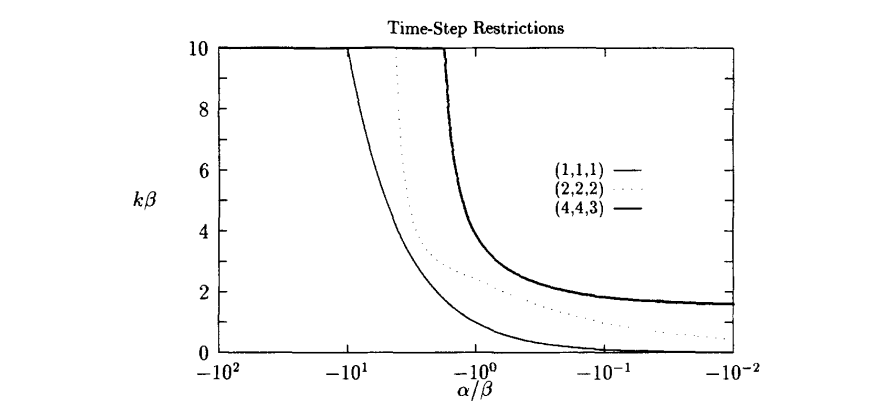
\includegraphics[width=15cm]{1.png}
\caption{对于满足(\ref{23})的IME-X格式,时间步长稳定性限制$\alpha$和$\beta$的值。在高衰减极限中这些格式都表现良。}
\centering
\label{figures1}
\end{figure}
\begin{figure}[H]
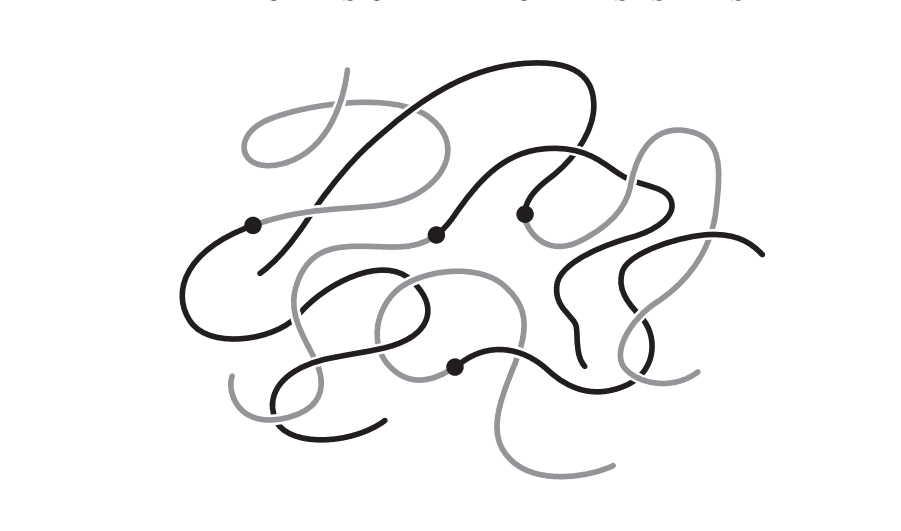
\includegraphics[width=15cm]{2.png}
\caption{对于满足(\ref{22})的IMEX方案,时间步长稳定性限制$\alpha$和$\beta$的值。其中一些格式,特别是(3,4,3),在$-\alpha$不太大的范围内表现良好,但它们在高衰减极限时都有时间步长限制。}
\centering
\label{figures2}
\end{figure}

图(\ref{figures2})中所有格式的共同点是,当$\alpha\to -\infty$有一个时间步骤限制涉及$\beta$,特别的$k\beta<1$,相反,对于满足图(\ref{figures1})中的(\ref{23})和(\ref{24})的格式没有这种限制。后一种格式在高衰减极限与SBDF格式的定性相似[2]。 另一方面,图(\ref{figures2})中的格式(3,4,3)在可允许的时间步长上体现了大范围参数值上的潜在优势。

\section{一维有限差分逼近}
\subsection{线性问题}

考虑一维变系数问题
\begin{equation}
u_{t}+sin(2\pi x)u_{x}=\nu u_{xx}
\label{41}
\end{equation}
区间[0,1]上的周期边界条件和初始条件
\begin{equation*}
u(x,0)=sin(2\pi x)
\end{equation*}
对于空间导数,我们使用二阶中心差分。对于所有$\nu\ge 0$,该解都是光滑的。

\subsubsection{大粘度的例子}

为了研究大粘度情况下IMEX RK格式的行为,用时间步长$k=1.8h_{0},h_{0}=\frac{1}{63}$逼近了模型问题(\ref{41})。对于空间离散,我们选择了$h=h_{0},h_{0}/2,h_{0}/4,h_{0}/8$的网格间距。利用几种格式,对粘度$\nu$在$0.01\le \nu\le 0.1$范围内进行了时间$t=2$的计算。对于$h=h_{0}$,这些值对应于网格雷诺数R,在$1.59\ge R\ge 0.159$的范围内。 对于较小的$h,R$相应地更小。

在最大范数中测量的相对误差在图(\ref{figures3})中相对于$\nu$绘制。在图3(a)中,省略了三级和四级格式的误差,因为它们总是在两级二阶格式(2,3,2)的2倍之内。正如上一节理论所预期的那样,当$\nu$较大时,三级DIRK(3,4,3)和满足性质(\ref{23})的格式允许更大稳定时间步长。
\begin{figure}[H]
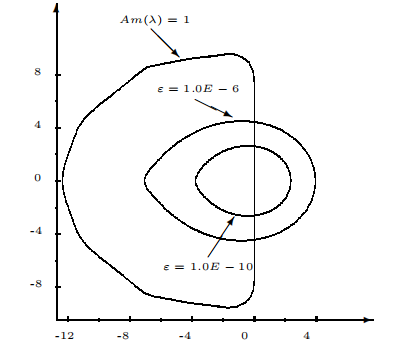
\includegraphics[width=15cm]{3.png}
\caption{$k=1.8h_{0},h_{0}=\frac{1}{63}$的大粘度行为}
\centering
\label{figures3}
\end{figure}

当我们降低$h$,保持k不变时,方法(1,2,2),(2,3,3)和(2,3,2)在整个$\nu $内变得不稳定。在稳定的方法中,空间误差不再控制时间误差在高阶(3,4,3)和(4,4,3)中更明显。对于$h=h_{0}/8$只有满足(\ref{23})的方法才能保持稳定。对于h和k的这些值,没有检测到有效的误差减少。
\begin{figure}[H]
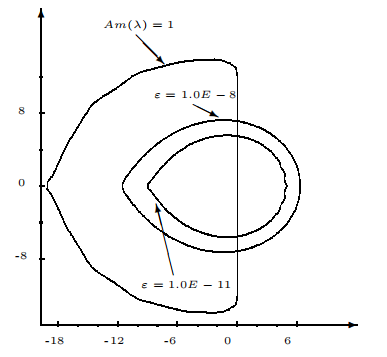
\includegraphics[width=15cm]{4.png}
\caption{$k=5.4h,h=h_{0}$的大粘度行为}
\centering
\label{figures4}
\end{figure}

在保持$h=h_{0}$的同时加倍时间步长也导致二级方法(2,3,2)和(2,3,3)在$\nu$整个区间内变得不稳定。 尽管如此,三级和四级方法在整个区间内保持稳定,并且格式(2,2,2)在大部分区间内是稳定的。即使将时间步长增加三倍(见图(\ref{figures4}),三级和四级也适合于近似强阻尼流。实际上,与[2]的结果相比,本例中的三级方法(3,4,3)比步长为1/3的CNAB格式更精确和稳定,即使对于相对粗糙的步长k也是如此。

\subsubsection{小粘度实例}

为了研究大网格雷诺数的IMEX RK方法的性能,空间离散步长$h=\frac{1}{81}$和时间离散步长$k=1.8h$对例子(\ref{41})进行近似。使用几种IMEX格式,对粘度$\nu $进行时间$t = 2$的计算,其范围为\\$0.001\le u\le 0.01$这些值对应于网格雷诺数R,在$12.3\ge R \ge 1.23$的范围内。

这些计算的最大范数的相对误差在图(\ref{figures5})中相对于$\nu$绘制。在这里,我们发现三阶格式和二级二阶DIRK(2,3,2)的误差几乎一致,因为它们主要由空间离散产生。特别值得注意的是,这四种格式的误差总是小于[2]中考虑的两步IMEX格式的误差,即使采用了两倍的时间步长。

\begin{figure}[H]
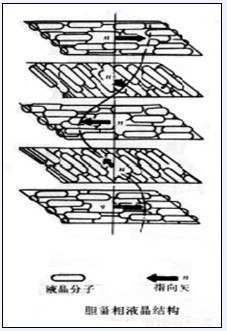
\includegraphics[width=15cm]{5.png}
\caption{$k=1.8h,h=\frac{1}{81}$的小粘度例子}
\centering
\label{figures5}
\end{figure}

\subsection{Burgers 方程}
对于Burgers方程,获得了与上面线性问题(\ref{41})定性相似的结果:
\begin{equation}
u_{t}+uu_{x}=\nu u_{xx}
\end{equation}
在齐次Dirichlet 边界条件和初始条件下,我们进行了实验
\begin{equation*}
u(x,0)=sin(\pi x),~~~0\le x\le 1.
\end{equation*}

对于小$\nu $,边界层在$x =1$附近发展。这就需要使用上风法。上风法可以看作是一个离散的$O(h)$扩散添加项(其中h是空间步长)$uu_{x}$一个中心差分逼近。

\section{二维中与时间相关的多重网格}

我们考虑二维对流扩散问题:
\begin{equation}
\mathbf{u}_{t}+(\mathbf{u}\cdot\nabla)u=\nu \Delta u,
\label{51}
\end{equation}
其中$\mathbf{u}\equiv (u,v)$。我们在方形$\varOmega\equiv [0,1]\times [0,1]$上进行计算并考虑周期边界条件和初始条件。
\begin{gather*}
u(x,y,0)=sin[2\pi (x+y)]+0.005cos[2\pi (64x+63y)],\\
v(x,y,0)=sin[2\pi (x+y)]+0.005cos[2\pi (64x+63y)],
\end{gather*}

对于空间离散,我们使用标准的二阶中心差分。时间步长是使用各种IMEXRK格式(对流项,$(\mathbf{u}\cdot\nabla)\mathbf{u}$是显式处理的,扩散项$\nu \Delta\mathbf{u}$是隐式处理的)。这种处理产生了一个正定的、对称的、稀疏的、线性的系统在每一步都要求解.采用多重网格算法有效地解决了这类系统的问题,并在[2]中给出了该算法的组成。

模型问题(\ref{51})使用网格尺寸$h=\frac{1}{128}$和每步$TOL=0.003$的剩余容量来近似。选择时间步长为$k=0.00625$取得了稳定的结果。对于几种IMEXRK格式,计算每个时间步的平均细网迭代次数。表1中提供了$v(1,1)$环的结果。除了第2节中提出的格式之外,我们还包括Griepentrog格式[6,7]的结果,它不是形式(21)。

\begin{figure}[H]
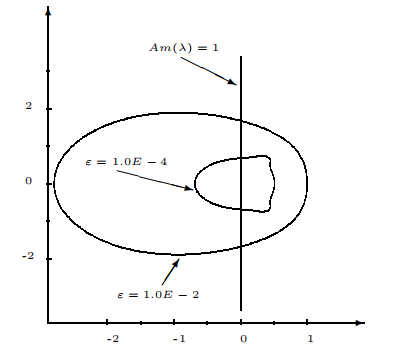
\includegraphics[width=10cm]{6.png}
\centering
\label{Table1}
\end{figure}

从表中可以看出,强阻尼L-稳定格式对于大粘度问题每阶段所需的细网格迭代次数最少。弱阻尼格式需要更多的努力来求解隐式方程的精确,因为挥之不去的高频模式需要在最精细的网格上进行。这对于隐式-显式中点格式(1,2,2)尤其明显,因为当$\nu >0.03$时,每阶段需要三次以上的迭代。Griepentrog的格式还需要额外的精细网格迭代,大概是为了抑制在初始阶段出现的高频成分。

\end{document}